\newpage
\section{Refactoring et révision de l'interface graphique}

\subsection{Révisions générales sur le code}
\paragraph{}
Nous avons rapidement établi que le refactoring du code existant
faisait partie des besoins de notre projet. Dans cette partie, nous
décrirons l'ensemble des travaux réalisés dans ce cadre.

\subsubsection{Conventions de programmation et assistance au programmeur}
\paragraph{}
L'un des premiers reproches faits par l'équipe pédagogique à
l'architecture héritée de Jérémy Lixandre est son manque de clarté ;
le code livré était trop peu commenté pour permettre à un programmeur
de comprendre ne serait-ce que le rôle de chaque classe sans rentrer
en détail dans l'intégralité de leur code. Pour cette raison, nous
avons abondemment commenté le code en rajoutant également de la documentation
doxygen. Pour tous les fichiers sources, nous trouvons dans l'en-tête de chaque
début de fichier \verb!.cpp! le rôle et le fonctionnement de ceux-là.
\paragraph{}
Des commentaires ont également été ajoutés massivement au niveau des
fonctions principales du programme. En effet, la compréhension du
programme existant a considérablement ralenti le démarrage de notre
implémentation sur ce projet, et a nécessité plusieurs recherches sur
le web et la consultation conjointe de divers documents de sources
différentes. Les deux fichiers ayant été les plus commentés de la
sorte sont \verb!main.cpp! et \verb!render.cpp!.
\paragraph{}
La syntaxe du code a été remodelée de manière générale pour répondre à
des conventions autant que pour faciliter sa compréhension : les
"include" en début de fichiers ont été classés selon le type de
fichiers inclus et par ordre alphabétique, la langue des commentaires
a été uniformisée, les indentations, choix de placement de
crochets/accolades etc. ont été uniformisés également pour une
meilleure cohérence de la syntaxe, les variables ont été renommées
pour être plus claires et éviter de heurter les conventions qui nous
ont été enseignées.

\subsubsection{Modification de l'architecture logicielle}
\paragraph{}
D'autres approches du code réalisées par Jérémy Lixandre nous
semblaient maladroites. Afin de rendre une architecture répondant au
mieux aux conventions de programmation vues en cours et qui soit la
plus compréhensible et claire possible aux yeux d'un potentiel futur
programmeur, nous avons apporté plusieurs révisions liées à
l'organisation des fichiers.
\begin{itemize}
 \item Le code de \verb!main.cpp! a été entièrement révisé. En effet,
       il contenait une unique fonction
       \verb!main(int argc, char *argv[])! qui nous paraissait bien trop
       dense. Afin de faciliter la compréhension du lecteur et de mieux
       correspondre aux conventions, nous avons effectué un découpage
       fonctionnel de cette fonction en plusieurs fonctions. La fonction
       \verb!main! appelle une fonction
       \verb!launch(int argc, char *argv[])! qui elle-même appelle
       d'autres fonctions (lesquelles, parfois, en appellent elles-mêmes
       de nouvelles).

       \begin{lstlisting}[language=C, frame=single, breaklines=true]
static void launch(int argc, char *argv[]){
  ChSettings gChSettings;
  Parser config;
  void *handle;
  ProcessMultiCorrel *p;
  config = initParser(argc, argv);
  handle = initHandler();
  p = initProcessMultiCorrel(handle);
  setupSettings(gChSettings, config, p, handle);
  initAndRun(gChSettings, config, argv);
  stopAndCleanupAudio();
  freeAndClose(gChSettings, config, p, handle);
}
 \end{lstlisting}

 \begin{center}
  \textit{Ci-dessus, le code de la fonction launch}
 \end{center}

 \item Nous avons de même effectué un découpage fonctionnel sur la
       fonction \\ \verb!bool setup!  du fichier \verb!render.cpp!. Ce
       fichier, qui présentait tout comme \verb!main.cpp! une
       organisation assez condensée, ne pouvait pas cependant être
       remanié autant en profondeur dans son intégralité que le code
       précédemment abordé. En effet, la fonction principale du
       fichier, \verb!void!  \verb!render!, ne pouvait être découpée de
       manière maintenable. En effet, elle exécute une boucle de
       traitement audio, en créant des taches auxiliaires exécutées par
       d'autres threads pour garantir un traitement rapide (qui doit
       être au minimum plus rapide que la vitesse de lecture des
       pistes), et il n'était pas possible de la découper sans créer de
       conflits sur les variables enregistrant le nombre de tours de
       boucle ou les variables contenant les signaux audio par exemple.

       \begin{lstlisting}[language=C, frame=single, breaklines=true]
bool setup(BelaContext *context, void *userData) {
  gUserSet = *((ChSettings *)userData);
  initUserSet(gUserSet);
  initBuffers();
  initSampleStreams(gUserSet);
  printInfo();
  return initAuxiliaryTasks();
}
 \end{lstlisting}

 \begin{center}
  \textit{Ci-dessus, le code de la fonction setup}
 \end{center}

 \item \`{A} l'intérieur du dossier \verb!process!, les
       différents fichiers de traitement ont été classés par
       fonctions en quatre dossiers \verb!Coeff!, \verb!Color!,
       \verb!Preproc! et \verb!Mix!. \`{A} l'intérieur du dossier
       \verb!test!, les fichiers que nous avons implémenté pour tester les
       différentes fonctions du programme ont été classés de la même
       manière (Jérémy Lixandre n'avait pour sa part pas implémenté
       de fichiers de test). Le fichier TestMain contenu à la racine du
       dossier test se chargera de récupérer le registre de l'ensemble
       des tests contenus dans les différents dossiers.

 \item D'une manière générale, les fichiers ont été triés pour
       ordonner l'architecture proposée par Jérémy qui était un peu
       confuse ; des fichiers de code n'ayant rien à voir entre eux
       se côtoyaient au sein d'un même dossier, et l'architecture
       présentait une hiérarchie n'étant pas toujours en rapport
       avec celle que présente le logiciel. Pour ces raisons, nous
       avons partagé les fichiers en plusieurs sous-dossiers,
       notamment les fichiers sources et les fichiers d'en-tête au
       sein du dossier \verb!VisualImpro!, et nous avons modifié
       les fichiers Makefile en conséquence. Le fichier de
       configuration \verb!config.cfg! a notamment été déplacé dans
       un nouveau dossier \verb!bin!.

 \item Dans le code livré par Jérémy Lixandre, un dossier
       \verb!VisualImproExe! regroupait un fichier de
       configurations, les fichiers relatifs à NodeJS, un fichier
       html lié à l'affichage de la matrice graphique via le
       navigateur Mozilla Firefox et les fichiers sources C++
       permettant les manipulations nécessaires au lancement du
       programme VisualImpro. Nous avons implémenté un script
       bash voué à remplacer la majeure partie de cette
       architecture, le fichier \verb!VisualImpro.sh! placé dans
       le dossier \verb!bin!.
\end{itemize}
\paragraph{}
Dans la version précédente de l'exécutable (\verb!VisualImproExe!),
les tâches réalisées par le code C++ étaient les suivantes :
\begin{itemize}
 \item Copier les fichiers \verb!.wav! indiqués dans le fichier de
       configuration dans Bela,
 \item Créer une copie du fichier de configuration, et y modifier les
       chemins des fichiers \verb!.wav! pour que ceux-ci correspondent au
       système de fichiers de Bela,
 \item Copier la copie du fichier de configuration dans Bela,
 \item Lancement du serveur NodeJS avec le fichier \verb!server.js!,
 \item Ouverture d'un onglet (ou d'une nouvelle fenêtre) du
       navigateur Firefox,
 \item Connexion à Bela (en ssh) et lancement du programme
       VisualImpro,
 \item Si le programme reçoit un signal d'interruption (Ctrl-C),
       alors certaines tâches sont réalisées :
       \begin{itemize}
        \item Arrêt du programme VisualImpro,
        \item Arrêt du serveur NodeJS,
        \item Suppression des fichiers \verb!.wav! sur Bela,
        \item Rapatriement des logs vers le dossier \verb!VisualImproExe!,
        \item Suppression de la copie modifiée du fichier de configuration,
        \item Arrêt de l'éxécutable.
       \end{itemize}
\end{itemize}
\paragraph{}
Durant l'audit, le fait de réaliser des manipulations de fichiers de
configuration, ainsi que des transferts de fichiers ou des connexions
vers Bela à l'aide de fichiers C++ a été pointé du doigt. En effet,
cette façon de faire reposait sur des classes C++ annexes qui
effectuaient les manipulations de chaînes de caractères dans les
fichiers de configuration, et pour ce qui concerne le transfert de
fichiers et la connexion vers Bela, cela été réalisé à l'aide d'appels
à la fonction C \verb!int system(const char *command)!.
\paragraph{}
Réaliser toutes ces opérations à l'aide d'un script bash paraissait
beaucoup plus pertinent. Cela permet de se passer des différents
fichiers sources et d'en-tête C++, et de plus, il existe des commandes
bash permettant de réaliser ces manipulations de chaînes de caractères
de façon beaucoup moins lourde et fastidieuse.
\paragraph{}
En plus de reproduire le comportement de l'ancienne version de
l'exécutable, notre script bash \verb!VisualImpro.sh! permet de
choisir entre les deux versions graphiques maintenant disponibles. Il
suffit de préciser à l'aide d'une option (\verb!qt! ou \verb!firefox!)
quel affichage on souhaite obtenir.
\paragraph{}
Parmi les autres aspects de l'existant que nous avons tenu à réviser,
la classe \verb!utilities! posait problème dans le sens où elle
contenait un trop grand nombre de fonctions n'ayant rien à voir entre
elles. Nous avons tâché de réduire son contenu au maximum, et
actuellement, elle ne contient plus que deux fonctions utilisées par
les fichiers \verb!main.cpp! et \verb!render.cpp!, et son rôle est
véritablement celui d'une classe utilitaire pour les fichiers
principaux du programme. Les fonctions de traitement que contenaient
cette classe et nécessitaient son inclusion dans tous les fichiers du
répertoire \verb!process! ont été déplacées et réparties dans le code
pour éviter ces inclusions systématiques. Nous avons également crée
une classe \verb!RGB! en remplacement de la structure \verb!RGB! que
contenait \verb!utilities!. Elle regroupe également les fonctions
refactorées de l'ancienne classe \verb!triplet!.
\paragraph{}
Face au grand nombre de traitements de matrices dans le code, nous
avons choisi d'implémenter une classe \verb!Matrix.cpp! afin d'éviter
d'utiliser systématiquement des vecteurs de vecteurs de flottants,
procédé lourd en écriture et exigeant l'écriture de fonctions de
traitement de vecteurs de vecteurs. La nouvelle classe \verb!Matrix!
rassemble toutes les opérations sur les matrices nécessaires au
programme, en plus de divers constructeurs pour créer des matrices de
différents types selon différents paramètres. Classe
\textit{template}, \verb!Matrix! permet de créer des matrices
d'entiers, de flottants ou bien de triplets RGB.

\paragraph{}
L'implémentation de Jérémy Lixandre comportait une classe
\verb!ProcessMulti! dont héritaient les classes
\verb!ProcessMultiCorrel! et \verb!ProcessMultiWriteWav!, mais
l'héritage n'avait pas lieu d'être puisque la classe
\verb!ProcessMulti! en question définissait une fonction abstraite
\verb!process!, redéfinie dans ses deux classes filles et prenant en
paramètre une matrice de flottants (représentant les signaux d'entrée)
et une connexion. Or, la classe \verb!ProcessMultiWriteWav! sert à
créer des fichiers \verb!.wav! et ne recquiert aucune connexion. Nous
avons donc cassé l'héritage entre ces classes et supprimé la classe
\verb!ProcessMulti!.

\paragraph{}
Nous avons ajouté des fichiers d'en-tête pour tous les fichiers source
contenant les fonctions de traitement, afin de pouvoir utiliser ces
fonctions, dans les fichiers de test notamment, en incluant les fichiers
nécessaires. Les fonctions de traitement étaient auparavant copiées
dans la classe \verb!utilities!, mais lors du refactoring de cette
dernière, nous avons réalisé que cette solution n'était pas très
conventionnelle.

\begin{figure}[H]
 \centering
 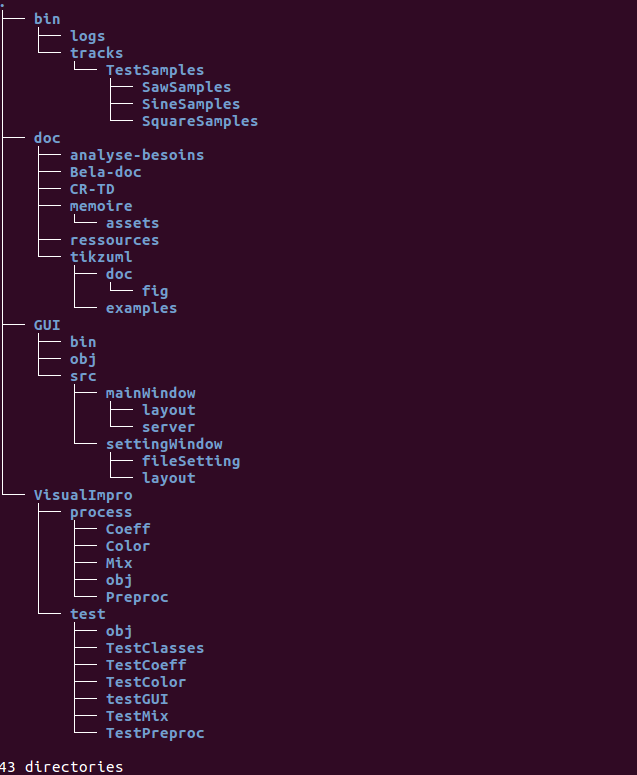
\includegraphics[scale=0.5]{assets/tree.png}
 \caption{Arborescence des fichiers}
 \label{schéma global}
\end{figure}

\paragraph{}
Voici ci-dessus l'arborescence de nos fichiers.


\subsubsection{Optimisation du code}
\paragraph{}
Afin de garantir un traitement rapide des informations par BELA et de
produire un retour sonore sans risque de latence, nous avons dû
optimiser certaines parties du code. Dans son rapport, Jérémy Lixandre
avait précisé que le traitement de BELA occupait une part trop
importante du CPU à partir de quinze fichiers \verb!.wav! traités
simultanément ; ce constat nous a encouragés à optimiser le programme
pour limiter le coût de son exécution.
\paragraph{}
L'implémentation de l'existant présentait notamment de nombreuses
copies des matrices passées en paramètres. Ces matrices sont des
éléments particulièrement lourds, contenant un nombre de données égal
au produit du nombre de pistes sonores en entrée par 32768 (taille des
buffers traités). Nous avons choisi de remplacer ces copies
successives de matrices par le placement en paramètres de références
constantes de ces matrices.

\begin{lstlisting}[language=C, frame=single, breaklines=true]
void ProcessMultiCorrel::process(const Matrix<float>& buffer,
                                 vector<float>& meanCorrelations,
                                 Connection conn){
  Matrix<float> copy = buffer;

  // Processing functions
  copy = _preprocess(buffer);
  Matrix<float> correlMatrix = calcul_correl(copy);
  process_volume(correlMatrix, meanCorrelations);
  Matrix<RGB> mat = color_matrix(correlMatrix);

  // Send data
  string str = mat.toString();
  conn.send(str);
}
\end{lstlisting}
\begin{center}
 \textit{Ci-dessus, la fonction principale de
  \verb!ProcessMultiCorrel.cpp!. Ce code témoigne de multiples
  opérations de refactoring et d'optimisations du code ; en effet,
  le nombre d'appels de fonctions au sein de la fonction process témoigne du
  découpage fonctionnel de la fonction d'origine, laquelle était autrement
  plus dense. De plus, on peut observer dans les paramètres qu'un
  vecteur des moyennes de coefficients de corrélation a été ajoutée
  pour permettre l'implémentation du mixage du retour sonore. Enfin,
  la matrice de flottants "buffer" a été changée en sa référence
  constante, afin d'éviter d'avoir à en faire une copie dans le
 corps de la fonction.}
\end{center}

\paragraph{}
Au sein de la nouvelle classe \verb!RGB!, de nombreux calculs notamment ceux permettant la conversion d'entiers en valeurs hexadécimales ont été simplifiés.

\subsection{Les changements apportés à l'interface graphique}
\paragraph{}
Précédemment, nous parlions de la nécessité de modifier l'affichage de
l'interface graphique pour diverses raisons. Nos clients n'exprimaient
pas de préférence quant à la méthode employée pour afficher la matrice
imaginée par nos prédécesseurs de l'ENSEIRB, mais nous trouvions peu
judicieux et coûteux pour le programme de passer par NodeJS et Mozilla
Firefox pour la produire. Un affichage graphique implémenté en C++
grâce au framework Qt nous paraissait plus logique, judicieux et
conforme au reste de l'architecture de notre programme.
\paragraph{}
Cependant, nous pouvons reconnaître l'avantage que peut avoir
l'affichage de la matrice sur un navigateur répandu comme Mozilla
Firefox. En effet, on peut imaginer qu'à l'avenir, le programme
embarqué sur le système Bela pourra se passer d'un ordinateur pour
fonctionner et afficher la matrice sur l'écran d'un smartphone par
exemple en passant par un navigateur web. Pour cette raison, nous
avons décidé d'offrir à l'utilisateur la possibilité de choisir entre
l'affichage Qt et l'affichage sur navigateur au moment de lancer
l'exécution du programme.

\subsubsection{L'implémentation de la méthode d'affichage sous Qt}
\paragraph{}
\`{A} l'intérieur du dossier \verb!GUI! répertoriant les classes
dédiées aux affichages graphiques, le dossier \verb!mainWindow!
contient l'architecture propre à l'affichage de la matrice graphique
via Qt. Elle contient une classe, \verb!GUIWindow!, et deux
répertoires : \verb!layout! dédié à l'affichage de la matrice, et
\verb!server! contenant le serveur établissant la communication avec
BELA.
\paragraph{}
L'architecture \verb!mainWindow! a pour unique rôle d'afficher la
matrice graphique de corrélations et de la mettre à jour en temps
réel. Elle réagit aux mises à jour transmises par BELA via
\verb!render.cpp! à l'aide de d'une connection TCP
et hérite de la classe Qt \verb!QMainWindow! ce qui
lui permet notamment d'afficher des menus. \`{A} l'avenir, ces menus
pourront permettre à l'utilisateur de modifier des configurations du
programme en temps réel si un successeur implémente cette
fonctionnalité.

\begin{figure}[H]
      \centering
      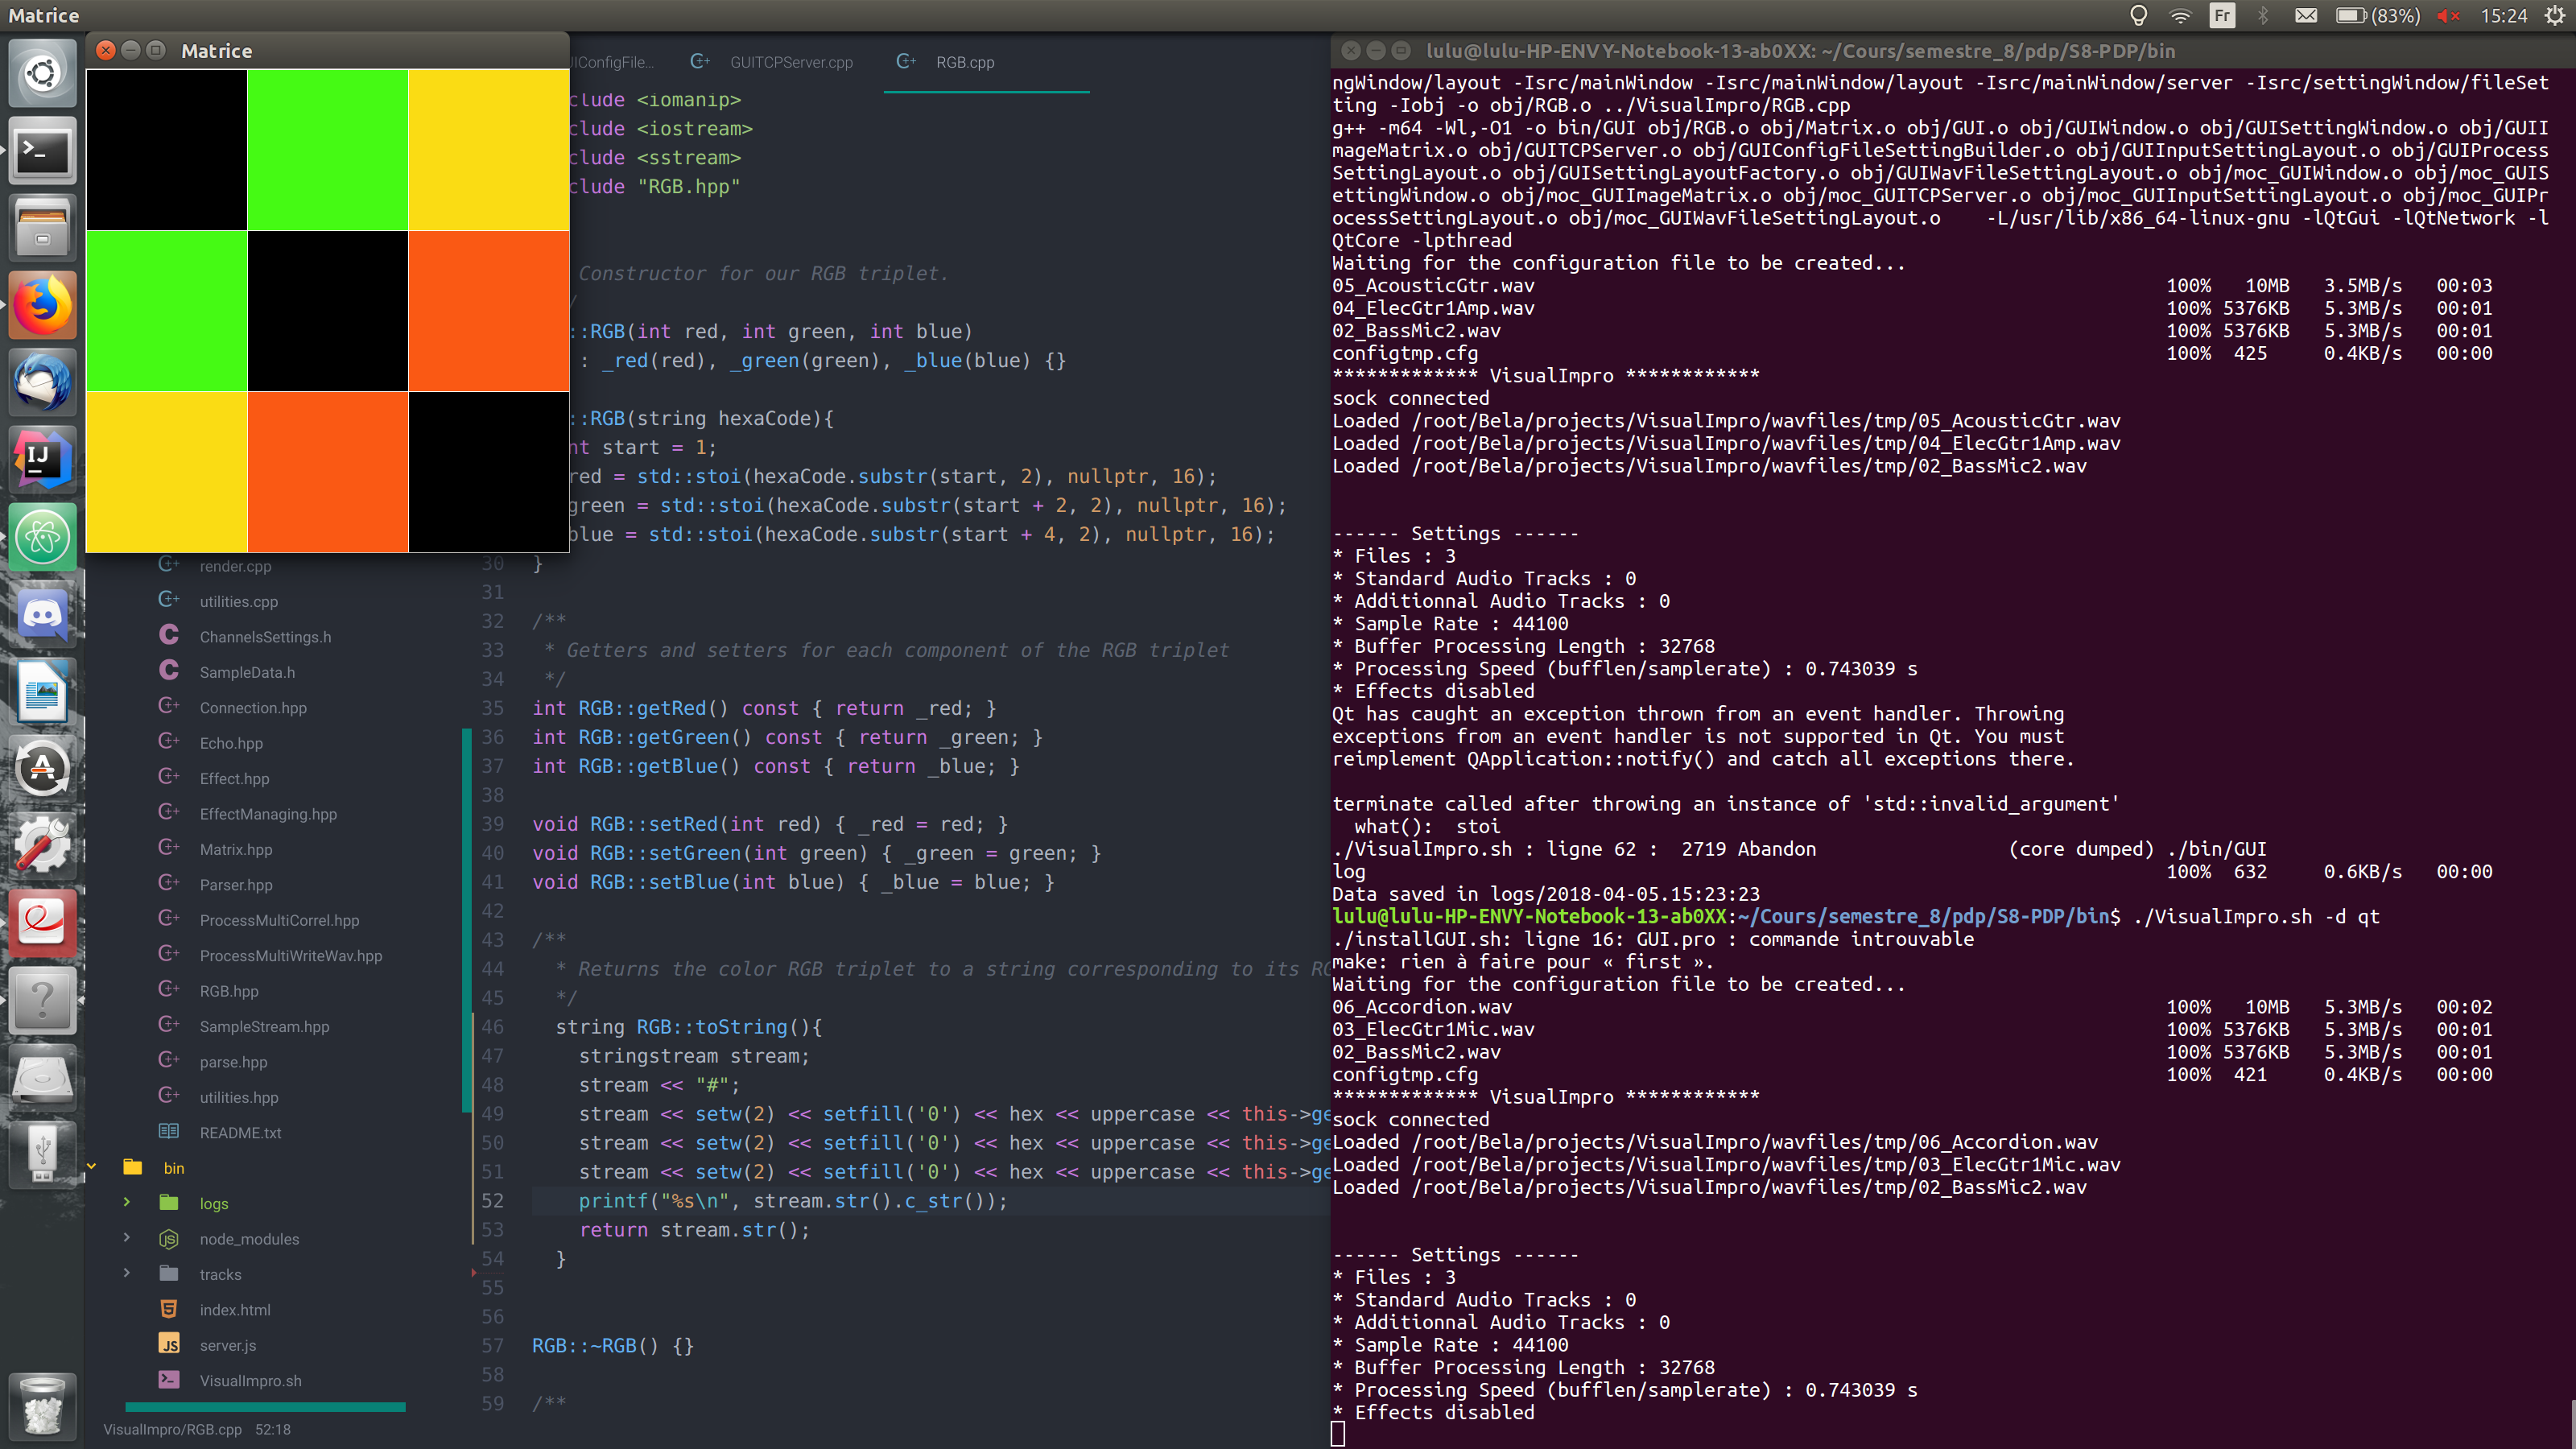
\includegraphics[scale=0.4]{assets/captureRGB.png}
      \caption{Aperçu de la matrice de corrélation affichée avec Qt}
      \label{principe général}
\end{figure}

\paragraph{}
La classe \verb!GUIImageMatrix! du répertoire \verb!layout! contient
un objet de type \verb!QPixMap! dont les couleurs sont mises à jour
pour chaque rectangle le composant.

\paragraph{}
La classe \verb!GUITCPServer! du répertoire \verb!server! constitue un
serveur TCP permettant la communication avec BELA. BELA se connecte a ce
serveur et crée une socket ; les paquets transmis par BELA et
contenant une matrice codée sous forme d'un objet de type
\verb!string! sont retraduits en matrice RGB. Le framework Qt permet
la communication entre le \textit{layout} et le \textit{server} via
l'émission de signaux depuis le serveur, transmettant les données de
la matrice à \textit{layout}.

\paragraph{}
Comme cette méthode d'affichage contient uniquement un serveur et un affichage
de matrice via une image, le programme se retrouve
extrêmement allégé par rapport au programme de notre prédécesseur qui utilisait Mozilla Firefox ainsi que NodeJS.
